% =========================================================
% main.tex  -  arXiv-ready article template (CS categories)
% =========================================================
\documentclass[11pt]{article}

% ---------- page geometry & style----------
\usepackage[margin=1in]{geometry}
\pagestyle{empty}

% ---------- fonts & encoding ----------
\usepackage[T1]{fontenc}   % decent PDF copy/paste
\usepackage[utf8]{inputenc}
\usepackage{lmodern}       % Latin Modern = vector version of Computer Modern

% ---------- math & symbols ----------
\usepackage{amsmath,amssymb,amsfonts,amsthm}
\newtheorem*{remark}{Remark}

% ---------- graphics ----------
\usepackage{graphicx}      % \includegraphics
\usepackage{subcaption}    % optional subfigures
\usepackage{tcolorbox}
\usepackage{placeins}
\usepackage{float}
\usepackage{booktabs}
\usepackage{enumitem}

% --- macros used in the information-theoretic bound ---
\usepackage{amsmath,amssymb}   % (already loaded in many templates)

\newcommand{\Err}{\mathrm{Err}}
\newcommand{\Prb}{\mathbb{P}}  % avoid \Pr: clashes with TeX primitive
\newcommand{\kappabar}{\bar{\kappa}}
\newcommand{\E}{\mathbb{E}}

% ---------- bibliography ----------
% Author-year (ACL-like)
\usepackage[
  backend=biber,
  style=authoryear,
  natbib=true,      % enables \citep / \citet
  maxbibnames=6,
  minbibnames=1,
  maxcitenames=2,
  sorting=none
]{biblatex}
\addbibresource{refs.bib}

% --- link BOTH author block and year in parenthetical cites ---
\DeclareCiteCommand{\citep}[\mkbibparens]
  {\usebibmacro{prenote}}
  {%
    \ifthenelse{\value{citecount}=1}
      {\bibhyperref{\printnames{labelname}\addcomma\space\printfield{year}}}
      {\bibhyperref{\printnames{labelname}\addcomma\space\printfield{year}}}%
  }%
  {\multicitedelim}
  {\usebibmacro{postnote}}
% --------------------------------------------------------------

\setlength\bibitemsep{1.0\baselineskip}


% ---------- theorem environments (optional) ----------
\usepackage{amsthm}
\newtheorem{definition}{Definition}
\newtheorem{lemma}{Lemma}
\newtheorem{theorem}{Theorem}

% ---------- custom macros ----------
\newcommand{\WriteCost}{\mathrm{WriteCost}}

% ---------- title data ----------
\title{The Courtroom Challenge—A Conjecture on the Unavoidable Cost of LLM Verification}
\author{John Repsys\thanks{email: john.repsys@gmail.com}}
\date{\today}

% ---------- hyperlinks ----------
\usepackage[colorlinks=true, linkcolor=black, citecolor=blue, urlcolor=magenta]{hyperref}

% =========================================================
\begin{document}
\maketitle
\begin{abstract}
Large-scale generative models hallucinate, and ad hoc patches hide the true cost of verification. We pose a falsifiable ultimatum: automate validation, prove it unnecessary, or pay the explicit human-in-the-loop bill. We conjecture that for any unbounded open-world data stream with Shannon entropy rate $h>0$, a system that lacks both a persistent precedent store and a friction-priced validation loop will accumulate unbounded prequential regret. To test this “validation trilemma” we formalise a state machine, a cost ledger, and an impossibility triangle, then invite the community to break it. A 100-query toy stream illustrates how the ledger is logged; optimising the validator is left to future work. We also introduce the Courtroom Model, a wrapper that subjects every claim—textual, visual, or otherwise—to precedent search, automated semantic checks, and selective escalation to an external judge. Each output is checked against persistent vector memory, and conflicting evidence reopens prior “case law.” The challenge stands: thrive without paying the validation bill—or show why the bill is inescapable.
\end{abstract}

\footnotetext[1]{Baseline script and toy data: \url{https://github.com/johnrepsys/courtroom-model}}


\section{Introduction}
\label{sec:intro}
Large Language Models (LLMs) have demonstrated impressive capabilities in generating context-rich outputs by associating patterns from large corpora. However, this power comes with a critical limitation: LLMs often produce plausible-sounding but factually incorrect conclusions, a phenomenon known as hallucination \citep{marcus2020nextdecade,shinn2023reflexion}. Without structured verification, these errors risk being perpetuated and even amplified over time, undermining trust in LLM-generated knowledge. Addressing this issue requires a system that not only generates associations but rigorously validates and refines them.
Throughout this paper we use the term
\emph{Courtroom} metaphorically: it denotes an epistemic due-process layer that challenges and verifies LLM outputs, not a system for practicing law or adjudicating legal disputes.

To address these shortcomings we pose the \textit{Courtroom Challenge}: a
hybrid state machine in which every LLM claim is tested against a persistent
precedent store and—when automatic checks falter—escalated under a
tunable \textit{validation\_preference} dial (formal spec in
Section~\ref{sec:framework}).  The design rewires known parts
(generator, retrieval, human oversight) but prices each byte, cycle,
and minute of validation.  Retrieval-augmented generation (RAG) provides the raw materials
\citep{lewis2020rag,fan2024ragsurvey}.  
Recent advances—Self-RAG's self-verification \citep{asai2024selfrag}, 
Iter-RetGen's retrieval-generation synergy \citep{shao2023iterretgen}, 
MemoRAG's compressed long-term memory \citep{qian2024memorag}, and 
Chain-of-Verification RAG's answer-driven re-checks \citep{he2024covrag}—motivate 
our persistent precedent store but still validate only per answer.  
Human-alignment work such as Constitutional AI 
\citep{bai2022constitutional} motivates the escalation branch.  
Whereas MemoRAG retains past evidence without auditing it, our buffer makes
each accepted verdict both permanent and costly.
Unlike debate frameworks \citep{chen2024reconcile,madaan2023selfrefine} or formal
provers \citep{wang2025malot}, we emphasise continuous cross-session
verification: knowledge is never final, only current.

\paragraph{Why a conjecture first?}
Well-posed problems often precede the data needed to solve them.  We
therefore publish the validation trilemma now: automate open-world
verification, prove it unnecessary, or price human judgment honestly.
Curves can wait until the target is unambiguous.

\paragraph{Scope and contribution.}
This is a conjecture note—\emph{no curves, by design}.  We provide a
falsifiable protocol and open-source meta-configuration so that anyone can
measure cost-adjusted regret.  Generators are already benchmarked; the
Courtroom Challenge benchmarks verification.  We invite the community
to break the conjecture or beat the baseline and thereby close the last
mile in trustworthy AI.

\section{The Courtroom Model: Legal Precedent \& Debate}
\label{sec:courtroom}
Humans think by generating ideas and challenging them. In scientific and philosophical inquiry, ideas are not just created—they are debated, tested, and refined. As discussed in Section~\ref{sec:intro}, the Courtroom Model integrates LLMs for idea generation, FAISS/Parquet for memory, and feedback loops for validation. In this section, we'll explore how these elements interact in greater detail.

Once an LLM generates an idea, it enters the 'courtroom'—where it is tested against structured precedent and subjected to rigorous debate. Ideas are challenged and refined, ensuring that only those that withstand scrutiny are accepted as truth. The Courtroom Model keeps every claim—new or old—under continual scrutiny, revising or discarding assumptions as fresh evidence arrives and thereby maintaining an evolving knowledge base rather than a static one.

Picture cumulative human knowledge as the area under a quarter-circle frontier. LLM association pushes the curve outward; the Courtroom validator folds it inward wherever new evidence pierces old beliefs. Expansion and maintenance run in lock-step, keeping the frontier smooth instead of ballooning into noisy bubbles. The prequential-regret metric defined in Section~\ref{sec:performance-measures} is the algebraic mirror of this movie: outward growth reduces error, but only if the validator's inward checks prevent unchecked drift.

The Courtroom Model introduces a hybrid framework that distinguishes itself from current AI methodologies by integrating associative reasoning (LLMs) with the persistent structure of legal precedents (FAISS/Parquet) and dynamic friction-priced validation (see Figure~\ref{fig:courtroom}).
This combination enables the model to adapt, incorporate external judgment, and apply continuous scrutiny—features largely absent in systems like ReConcile or MA-LoT.

Rather than requiring manual review of every idea, the Courtroom Model automatically flags associations that meet certain thresholds of uncertainty or inconsistency with established facts. This approach allows humans to focus on the most critical evaluations, ensuring that their intervention is directed toward areas where it adds the most value.

\begin{figure}[H]
  \centering
  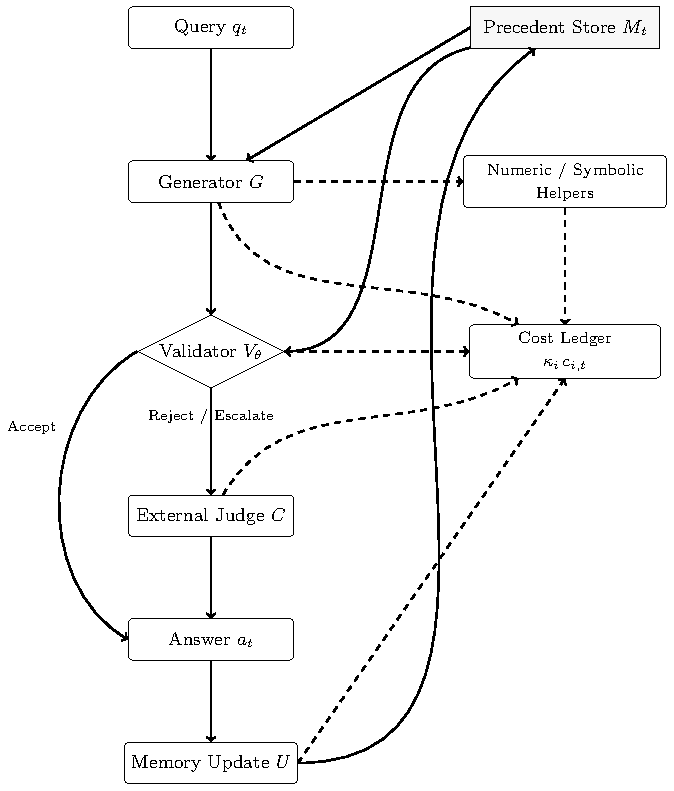
\includegraphics[width=0.9\linewidth]{figs/courtroom}%
      % no .pdf extension needed if LaTeX finds courtroom.pdf
  \caption{One step of the Courtroom loop.%
           \ Solid arrows: primary query flow.%
           \ Dashed arrows: helper calls and cost logging.%
           \ The cost\,bus aggregates all resource writes into a single ledger.
           \ On \textsc{DEFER} the round is skipped (no cost, no memory write).
           \ If C cannot supply an authoritative value—because the fact is genuinely unknown—the 
           \ query transitions to a terminal UNRESOLVED state; no memory write occurs.}
  \label{fig:courtroom}
\end{figure}

% ---------- quick-reference box ------------------------------------
\begin{tcolorbox}[colback=black!3,colframe=black!40,
  boxrule=0.4pt, arc=2pt, left=2pt, right=2pt,
  top=4pt, bottom=4pt, title=Notation snapshot]
\small
\begin{itemize}[leftmargin=*]
\item $G$ - \textbf{Generator}: LLM (+ optional helper calls)
that proposes a hypothesis $h_t$ for query $q_t$.
\item $V_{\theta}$ - \textbf{Validator} with
\emph{validation-preference dial} $\theta\!\in[0,1]$  
($0 =\,$speed‐first, $1 =\,$accuracy‐first).  
The dial is fixed during any evaluation run; see
Sec.~\ref{sec:framework}.
\item $\kappa_i c_{i,t}$ - \textbf{Cost-ledger term}: each resource $i$
(bytes written, CPU‐seconds, human minutes …) is logged as a
quantity $c_{i,t}$ weighted by its unit cost $\kappa_i$.
$\sum_i\kappa_i c_{i,t}$ is the friction paid at step $t$.
\item $\tau$ - \textbf{Retention threshold} that controls whether a
new descriptor vector is written to the precedent store:  
\vspace{-2pt}
\[
\text{write\_new}=\begin{cases}
[\cos\theta < \tau], &\text{(cosine form)}\\[4pt]
[\lVert x-y\rVert_2 > \tau], &\text{(distance form)}
\end{cases}
\]
Designers may substitute any monotone similarity metric.
\end{itemize}
\vspace{2pt}\par\footnotesize (Formal definitions → Section~\ref{sec:framework})\par
\end{tcolorbox}
% --------------------------------------------------------------------



\FloatBarrier



\vspace{1em}
\subsubsection*{Illustrative trace (informal)}

\noindent
\textbf{Query $q_t$.}  
\emph{``Wells Fargo's 2018 10-K introduces a line
\texttt{Debt securities}.  
(1) Map this line item to the existing FY-2017 bucket taxonomy, and  
(2) report the FY-2018 amount in that bucket.''}

\paragraph{1. Generator $G(q_t,M_t)\;\longrightarrow\;h_t$}
The precedent store $M_t$ has no FY-2018 descriptor for
\texttt{"Debt Securities"}.  
Embedding search ranks  
\texttt{(WFC, "Investment Securities", FY2017, 10.664 B)}  
as the nearest neighbour (high string similarity).
The embedding vector and its nearest neighbour are cached and handed to the validator in the same step.
Assuming the new label is merely a rename, the LLM—assisted by a local
XBRL helper that extracts the numeric value—relabels the bucket and
proposes  
\[
h_t=\text{``Bucket: \texttt{"Investment Securities"}; FY-2018 amount: \$10.664 B.''}
\]
The helper itself is numerically correct; the label choice is the error.

\paragraph{2. Validator $V_\theta(q_t,h_t,M_t)\;\longrightarrow\;$} ESCALATE
Using the same lookup result, the validator sees that the query descriptor  
\texttt{WFC\,$\vert$\allowbreak\,"Debt Securities"\,$\vert$\allowbreak\,FY2018} is only  
$\cos=0.906$ similar to its nearest neighbour  
\texttt{"Investment Securities"}.  
Because the illustration fixes the retention threshold at $\tau=0.95$, this
similarity falls outside the allowed neighbourhood, so the claim is
escalated—no domain-specific rule required.

\paragraph{3. External judge $C$}
A human analyst consults the 2018 10-K and confirms that
\texttt{Debt Securities} is a new line-item, not yet present in
the taxonomy.  The analyst extracts the FY-2018 amount  
\[
a_t = \text{``Bucket: \texttt{"Debt Securities"}; FY-2018 amount: \$14.406 B.''}
\]

\paragraph{4. Memory update $U(\dots)\;\longrightarrow\;M_{t+1}$}
Because \texttt{"Debt Securities"} represents a genuinely new bucket
(label and composition differ from \texttt{"Investment Securities"}),
$U$ appends a fresh descriptor vector
\texttt{WFC$\mid$"Debt Securities"$\mid$FY2018}\;→\;14.406 B.  
The existing \texttt{"Investment Securities"} tuples remain intact; an
optional \emph{alias edge} can later be added if domain experts decide
the two buckets should roll up to the same parent taxonomy node.

\paragraph{Cost ledger entry $\displaystyle\text{WriteCost}_t=\sum_i\kappa_i\,c_{i,t}$}

\begin{table}[h]
\centering\footnotesize
\begin{tabular}{@{}lccc@{}}
\toprule
Resource $i$ & Quantity $c_{i,t}$ & Weight $\kappa_i$ & $\kappa_i c_{i,t}$ \\ \midrule
Vector write (bytes)      & 1\,536 B & \,$1.0\times10^{-6}$ /byte & 0.0015 \\
FAISS rebuild (sec)       & 0.20 s   & 0.05 /s                 & 0.0100 \\
Human review (minutes)    & 1.00 min & 1.00 /min               & 1.0000 \\ \midrule
\textbf{Step cost}  & & &  \textbf{1.0115} \\ \bottomrule
\end{tabular}
\caption{Friction priced for this step (arbitrary $\kappa$-weights).}
\end{table}

\paragraph{Storage dial.}
The precedent store need not—indeed, should not—memorise every numeric
fact. A single \emph{retention knob} (\(\tau\)) decides whether a freshly
extracted descriptor vector is written back or simply reuses its nearest
neighbour. Let \(S(x,y)\) be any similarity score where “larger means
closer” (or equivalently a distance \(D(x,y)\) where “smaller means
closer”). The generic rule is

\[
\text{write\_new} =
\begin{cases}
\bigl[S(x,y) < \tau\bigr], & \text{(similarity form)}\\[4pt]
\bigl[D(x,y) > \tau\bigr], & \text{(distance form)}.
\end{cases}
\]

Cosine and L$_2$ are special cases, but a system designer is free to
plug in any monotone metric—e.g.\ Mahalanobis distance, dot-product in a
learned embedding space, or even a hybrid score that blends semantic and
numeric keys—so long as the inequality is flipped to match the
metric's notion of proximity. Section~\ref{sec:sparse-memory-bound-tightness} analyses the cost/error trade-off
under the distance form, and Appendix~\ref{sec:knobs} lists this dial
among the falsifiability-critical degrees of freedom. Selecting which descriptor 
fields to embed is itself tunable; Section~\ref{sec:open-questions} (Q\ref{open-question-schema}) sketches how the Courtroom loop 
could learn or prune schema columns over time.


\section{A Practical Implementation: Financial Data as a Reasoning Playground}
While much of the LLM + formal proof conversation focuses on pure math (e.g., Lean), the Courtroom Model has broad applications, including complex domains like financial data. In this space, ambiguity and structure meet, and semantic checks become crucial:
\begin{itemize}
    \item SEC filings often contain inconsistent naming and formats. LLMs can provide initial opinions on relationships between known metrics.
    \item Vector embeddings allow semantic similarity checks with prior precedent, using metrics such as L$_2$-distance or cosine similarity to quantify the closeness between new ideas and established knowledge. These checks focus on identifying close matches to validated concepts and flagging potential outliers, ensuring that the system not only finds similarities but also highlights discrepancies that might indicate the need for deeper scrutiny or re-evaluation.
    \item FAISS performs nearest-neighbor searches over high-dimensional vectors, helping to identify similar concepts based on predefined thresholds.
    \item Parquet files serve as version-aware memory, storing validated items, like legal precedent.
    \item In financial analysis, when a generative model suggests a correlation or metric, human analysts review it against historical data, verify the logic, and confirm its validity. This friction ensures errors do not become accepted facts.
\end{itemize}
This process embodies the Courtroom Model: association meets structure, refined and verified by friction. This perpetual validation loop not only updates the knowledge base as new data arrive; it also prioritises which claims to re-examine—triggered by real-world data, symbolic checks, human oversight, or similarity signals (e.g., cosine/L$_2$ distances)—so that older beliefs face deeper scrutiny whenever fresh evidence challenges them.
In practice, the model could leverage dynamic prioritization algorithms to determine which associations or precedents are most in need of re-evaluation. This approach would enable the model to scale effectively to large datasets, focusing scrutiny on the most impactful claims and reducing computational load while maintaining rigorous validation. While this is not yet implemented, it represents a key area for future development, enhancing the system's efficiency and scalability.

\section{Are LLMs a Dead End? Converging Error}
Critics such as LeCun \citep{LeCun2023SFI}\, argue that
purely autoregressive LLMs will always accumulate error:
if the per-token slip rate is $e$, the probability an
$n$-token answer is entirely correct decays as
$P_{\mathrm{correct}} = (1-e)^{n}$.
LeCun also notes the inability of LLMs to represent continuous high-dimensional spaces that characterize the real world, potentially limiting their ability to deal with complex, nonlinear data.

However, this does not mean we must abandon LLMs. Rather than expecting LLMs to handle everything on their own, the Courtroom Model allows them to excel at generating ideas and associations, while supplementing them with additional systems that anchor their outputs and guide them toward more reliable outcomes. By integrating persistent memory (like legal precedent) and real-world constraints (courtroom debate), the model offers a framework for continuously verifying and refining LLM-generated associations, ensuring they align with established facts and real-world data. This helps overcome challenges posed by complex, high-dimensional data, and can mitigate error propagation.

Meanwhile, the question “Are LLMs a dead end?” continues to evolve as part of the broader debate on AI's future. Some initially speculated that superintelligence was near, while others, like LeCun, pushed back, suggesting that LLMs' potential was overstated. The debate remains open—and that is exactly the point: we need friction to continue exploring ideas and improving models. The Courtroom Model offers one possible way forward by leveraging LLMs in combination with other systems, ensuring that we don't discard their value but integrate them into a broader framework that allows them to evolve meaningfully. While critics argue that LLMs have stalled AI progress, it may be more accurate to say that we're just learning to build one side of the brain, and as we expand our approach, we must continue building the other side as well.

\section{Multi-LLM Dialogues: An Interim "Court"}
\label{sec:multi-llm}
Several approaches have attempted to improve LLM reasoning through collaboration or debate among multiple agents. Systems like ReConcile \citep{chen2024reconcile} and Self-Refine \citep{madaan2023selfrefine} demonstrate that critical dialogue and iterative refinement between LLMs can enhance factual consistency and reasoning depth. However, these methods typically operate in a single-session paradigm, stabilizing on a consensus answer without maintaining a persistent knowledge base. In contrast, the Courtroom Model incorporates continuous precedent management, ensuring that knowledge evolves dynamically over time rather than resetting between tasks.

\section{Architectural Analogues}
\label{sec:analogues}
Structured exploration, exemplified by AlphaGo's policy-value search \citep{silver2016alphago} and more recently by Tree-of-Thoughts planning \citep{yao2023tree}, offers a compelling model for integrating creativity with systematic validation. In AlphaGo, a policy network generates moves, a value network evaluates outcomes, and self-play iteratively refines strategy. The Courtroom Model generalizes this principle to open-ended domains, applying continuous validation not only internally but also against a persistent external memory and, when needed, human oversight. This convergence supports the idea that the Courtroom Model is not prescriptive, but descriptive — a lens for recognizing effective reasoning architectures wherever they emerge. It offers a retrospective framework to describe such structures — and perhaps guide the design of future systems that balance creativity with constraint.

In formal mathematics, frameworks such as Lean \citep{mathlib2020lean} and multi-agent proof systems like MA-LoT \citep{wang2025malot} demonstrate that combining generative reasoning with strict verification pipelines can achieve rigorous correctness. These systems ensure that every step adheres to formal logic before being accepted. Inspired by these principles, the Courtroom Model aims to bring analogous rigor to less formally structured domains, using semantic similarity, precedent management, and a friction-priced external judge—human or automated—to prevent the unchecked propagation of errors.

Both AlphaGo and Lean + LLM workflows demonstrate that progress often arises from structured friction, not just creative leaps. In the same way, the Courtroom Model allows for creativity (via LLMs) to drive idea generation, but that creativity is continually tested and refined through structured validation and external challenge, ensuring only robust, verified ideas become part of the model's evolving knowledge.

\section{Open Questions}
\label{sec:open-questions}
\begin{enumerate}
    \item Is abstraction a distinct step in hybrid reasoning? When no exact precedent exists, does the model create a new one by compressing multiple associations? Should pattern recognition and abstraction be formal components in systems like this one?
    \item Can LLMs + real-world observation produce entirely new theories? If so, how do we detect genuine novelty, and how do we measure validity?
    \item Can the Courtroom Model generalize to other real-world domains and AI integrations? Healthcare, policy, engineering — any area that needs scale, creativity, and robust checks. Could this framework point toward a general pattern for hybrid AI?
    \item How can we achieve Lean-level formal rigor in open-text domains without relying solely on large LLM ensembles, whose granularity still falls short in many fields?
    \item \label{open-question-schema} How should the precedent store be schematised and evolved? Even in a well-defined vertical like finance, designing the descriptor schema (e.g.\ `(ticker, canonical\_metric, period, unit, GAAP\_flag, source\_tag, …)`) remains an art: too coarse results in semantic collisions; too fine results in unlimited vector growth. Can the system learn an optimal schema online—merging rarely-queried fields, splitting ambiguous ones, and doing so without breaking L$_2$-distance semantics? What signals (query regret, type-confusion rate, index rebuild cost) best drive such schema evolution?
    \item How do we maintain the tension between speed and scrutiny? Associative models want to generate rapidly; symbolic structures demand thorough verification. Speed wins until it fails. Scrutiny survives because it must.
    \item What does success look like in a system that's always evolving? As new precedents form, do we prune old ones? How do we adapt long-standing truths? The answer may lie in how far our energy limitations let us revisit and revise what we already hold to be true.
    \item Which self-play or adversarial-debate schemes could fill the \(V_\theta\) slot while keeping \(\kappa_{\text{compute}}\) at or below the current human-review baseline?
\end{enumerate}
\begin{tcolorbox}[colback=gray!5,colframe=gray!40,title=Why a concept note?]
  The field currently optimises ever-larger generators without a matching theory of
  validation.  We publish this abstraction before a prototype for two reasons:
  (i)~to surface hidden degrees of freedom that can silently invalidate benchmarks,
  and (ii)~to recruit empirical collaborators—open-sourcing code is planned for v2.
\end{tcolorbox}

\section{Toward Hybrid Intelligence}
\label{sec:hybrid-intelligence}
Purely neural stacks still stumble on reliability. Recent work \citep{marcus2020nextdecade, dawid2024latent} shows that scale alone cannot guarantee robust reasoning. This has revived calls for neuro-symbolic fusion: pair an associative generator with a structured verifier. The Courtroom Challenge operationalises that philosophy. It links:
\begin{itemize}
    \item an LLM's creative search,
    \item a persistent precedent memory, and
    \item an external judge (self-play agent, formal prover, ensemble LLM, or human),
\end{itemize}
into a single friction-priced loop that can correct itself over time. Reasoning at scale demands all three roles:
\begin{itemize}
    \item Generate \& explore — propose novel chains of thought.
    \item Validate \& prune — confront each claim with precedent, logic, and counter-evidence.
    \item Evolve the canon — admit only those claims that survive scrutiny, while logging the cost of that scrutiny.
\end{itemize}
Without this three-way handshake, knowledge either drifts (if validation is cheapened) or ossifies (if exploration is throttled). The Courtroom specification is therefore a minimal test-bed for hybrid intelligence: break the conjecture, or show how your system pays the validation bill more efficiently.

\section{Conclusion: A New Frontier}
\label{sec:conclusion}
Progress in reasoning systems emerges when every new idea must survive structured challenge. The Courtroom Model unites neural creativity, symbolic memory, and real-world friction in a single, continuously verifiable loop. By insisting that accepted knowledge remains open to appeal whenever fresh evidence appears, it transforms static retrieval or one-off debate into a living jurisprudence of facts. Future work will automate domain-specific validators and refine escalation thresholds, but the central thesis stands: reliable AI will look less like a confident oracle and more like an evolving court—where claims, evidence, and precedent are in constant, accountable dialogue.
If Conjecture~\ref{conjecture1} holds, genuinely autonomous, self-improving AI will require breakthroughs in scalable validation—pushing practical ASI timelines beyond what generator-only scaling curves imply.

\section{Minimal State Machine}
\label{sec:minimal-state-machine}
Formal state $S_t=(q_t,h_t,a_t,M_t)$, validator $V_\theta$, memory update
$U$, cost ledger $\WriteCost = \sum_i \kappa_i\,c_i$.
%
Validator actions:
$\{\textsc{ACCEPT},\textsc{REJECT},\textsc{ESCALATE},\textsc{DEFER}\}$.
%------------------------------------------------
\section{Formal Framework}
\label{sec:framework}
%------------------------------------------------

\subsection{State Spaces}
\label{sec:state-spaces}

\begin{itemize}\setlength\itemsep{2pt}
  \item Query space $Q$
  \item Hypothesis space $H$ (outputs of the LLM generator~$G$)
  \item Answer space $A$
  \item Memory space $M\subseteq\mathbb R^{d}$ (FAISS/Parquet vectors with payload)
\end{itemize}

As defined in Section~\ref{sec:minimal-state-machine}, state
\[
  S_t \;=\; \bigl(q_t,\; h_t,\; a_t,\; M_t \bigr), \qquad M_t\text{ finite}.
\]

\subsection{Components}
\label{sec:components}

\begin{itemize}
  \item \textbf{Generator.}  
  \(G : Q \times M \to H\) is an associative engine (e.g.\ an LLM) that proposes a
  hypothesis \(h_t\).  
  \(G\) may issue lightweight helper calls to numeric or symbolic libraries
  during exploration; such calls accrue \(\kappa_{\text{compute}}\) in the cost ledger
  but do not decide final truth.
  
  \item \textbf{Validator family.}  
  \(V_{\theta} : (Q, H, M) \to \{\textsc{ACCEPT}, \textsc{REJECT}, \textsc{ESCALATE}, \textsc{DEFER}\}\), with a
  tunable validation-preference dial \(\theta \in \Theta\).
  \(V_{\theta}\) may be
  (i) a stronger ensemble LLM,
  (ii) a formal-proof kernel,
  (iii) a deterministic numeric or symbolic tool-chain that certifies or refutes the claim, or
  (iv) a human panel as fallback.\footnote{\textit{Self-play precedent.}  
  AlphaZero's value network functions as an automated judge for Monte-Carlo rollouts.
  The Courtroom validator is its open-domain analogue: any module that can reliably
  downgrade faulty claims can occupy the judge slot.} \textsc{DEFER} means “skip this round”: no answer is returned,
  no escalation cost is paid, and the generator proceeds to the next
  query.
  
  \item \textbf{Memory update rule.}
  \(U : (M, q, h, a) \to M'\) records (or merges) a precedent whenever a claim is
  accepted.  Whereas vanilla RAG treats retrieved passages as a transient
  context window \citep{lewis2020rag}—and even iterative or self-reflective
  extensions still validate only the current answer
  \citep{shao2023iterretgen,asai2024selfrag}—the Courtroom store is
  persistent: it survives across sessions and every entry can later be
  re-audited for contradiction or obsolescence.

  \end{itemize}


\paragraph{Provisionality of verdicts.}
Even the external Judge's verdicts are provisional: they may be rescinded
if subsequent audits or new primary filings contradict earlier
conclusions.  Accordingly, Judge-validated precedents can be re-queued,
incur additional \(\WriteCost\), and overwrite prior entries via the usual
supersession mechanism.

\subsection{One--Step Transition}
\label{sec:transition}

Given $S_t=(q_t,h_t,a_t,M_t)$:
\begin{enumerate}
  \item $h_t \leftarrow G(q_t,M_t)$
  \item $d_t \leftarrow V_\theta(q_t,h_t,M_t)$
        \begin{itemize}
          \item If $d_t=\mathrm{ACCEPT}$ set $a_t=h_t$
          \item Else obtain corrected answer $a_t = C(q_t,h_t)$
                (oracle $C$ may call a human; cost is logged)
          \item If $d_t=\textsc{DEFER}$ set $a_t=\bot$
                and skip Steps 3-4 below.
        \end{itemize}
  \item $M_{t+1} \leftarrow U(M_t,q_t,h_t,a_t)$
  \item External stream provides $q_{t+1}$
\end{enumerate}

\subsection{Cost Ledger}
\label{sec:cost-ledger}

Let $c_{i,t}$ be the measured consumption of resource $i$ at step~$t$
(bytes written, FAISS rebuild time, human minutes, etc.).
Fix weights $\kappa_i$ once per benchmark—should the conjecture survive first contact.  The per-write cost is
\[
  \WriteCost_t \;=\; \sum_i \kappa_i\,c_{i,t}.
\]
Cumulative friction budget …  $F_T = \sum_{t=0}^{T-1}\WriteCost_t$.%
\footnote{\textsc{DEFER} incurs zero cost, so the corresponding
$\WriteCost_t$ entry is~0.}

\subsection{Performance Measures}
\label{sec:performance-measures}

Instant error
\[
  e_t = \mathbb{I}\bigl[a_t \neq \text{ground}(q_t)\bigr].
\]
Prequential regret after budget~$B$:
\[
  R(B) \;=\; \sum_{t=0}^{T(B)-1} e_t,
  \quad
  T(B) = \min\{\,T : F_T \ge B\,\}.
\]

\subsection{Setup}\label{sec:setup}

The definitions in \S\ref{sec:framework} merely fix notation
(\(T,\kappa,\Err,\theta,X\)); they do not restrict the validator's
internal design.  We now state Lemma~\ref{lem:ErrLower}, an
information-theoretic lower bound that applies to any interactive
validator whose transcript carries at most \(I\) bits of information
about the hidden label.  The inequality therefore functions as
motivation for the Courtroom architecture rather than a theorem
that assumes it.

\paragraph{Per-round notation.}
Fix a margin parameter $\delta\in(0,1]$.
For every run $\omega$ and round $t=1,\dots,T$ set
\begin{align*}
  y_t      &:=y_t(\theta)          &&\text{(ground-truth label)},\\
  h_t      &:=h_t(\omega)          &&\text{(validator's automatic prediction)},\\
  \mathrm{Esc}_t&:=\mathbf 1_{\{\text{round $t$ is escalated}\}.}
\end{align*}
Define the \emph{leverage rounds}
\begin{equation}\label{eq:kappaDef}
  \mathcal L(\omega):=\Bigl\{\,t:\,
     \mathrm{Esc}_t=0\;\text{and}\;|y_t-h_t|\ge\delta\Bigr\},
  \qquad
  \kappa(\omega):=\frac{|\mathcal L(\omega)|}{T}.
\end{equation}
The cumulative label error on those rounds is
\begin{equation}\label{eq:ErrDef}
  \Err(\omega):=\sum_{t\in\mathcal L(\omega)}
                \mathbf 1_{\!\bigl[h_t\neq y_t\bigr]}.
\end{equation}
Define the global means:
\[
  \bar\kappa:=\E[\kappa],
  \qquad
  \Err_{\mathrm{bar}}:=\E[\Err].
\]


\subsection{Information-theoretic lower bound}\label{sec:info-bound}

\begin{lemma}[Interactive-Fano corollary, general prior]\label{lem:ErrLower}
Let $V$ be any validator run for $T$ rounds.
With $\kappa(\omega)$ and $\Err(\omega)$ defined in
\eqref{eq:kappaDef}-\eqref{eq:ErrDef}, write
$\Err_{\mathrm{bar}}:=\E[\Err]$.
Assume the transcript $X$ obeys the information budget
$I(\theta;X)\le I$ under an arbitrary\, prior $\mu$ on the $M$-point label set $(M\!\ge\!2)$.
Define
\[
  H_{\star}:=
  \begin{cases}
      H(\theta) & \text{(Shannon entropy)}\\[4pt]
      -\log p_{\max} & \text{(min-entropy),}
  \end{cases}
  \qquad
  p_{\max}:=\max_{m}\mu(m).
\]
Then
\begin{equation}\label{eq:ErrLower-general}
  \boxed{\,%
   \Err_{\mathrm{bar}}
   \;\ge\;
   \frac{\delta\,T}{4}\;
   \kappa_{\!*}\;
   \Bigl(1-\tfrac{I+\log 2}{H_{\star}}\Bigr),
   \quad
   \kappa_{\!*}:=
     \E\bigl[\kappa\,\bigl|\,\Err>\tfrac12\delta\kappa T\bigr]
  \,}.
\end{equation}
\end{lemma}

\begin{remark}[Entropy convention]
Throughout we write $H_{\star}$ for whichever entropy measure is appropriate
in context—Shannon entropy when a prior is specified, min-entropy when no
distributional knowledge is assumed.
Uniform priors maximise $H_{\star}$, producing the strongest (largest)
version of the bound, while skewed priors reduce $H_{\star}$ and weaken the
barrier proportionally.
\end{remark}

\begin{proof}[Proof sketch]
Step 1 (separation).
For any $m\neq m'$ and transcript $x$ at most one of
$y_t(m),y_t(m')$ can equal $h_t$ on a leverage round, hence
\[
  \Err_m(x)+\Err_{m'}(x)\;\ge\;\delta\,\kappa(\omega)\,T.
  \tag{$\ast$}
\]

\noindent
Step 2 (interactive Fano). 
Set the path-dependent loss
\[
  L^\star(m,x)
    := \mathbf{1}_{\{\Err_m(x)>\tfrac12\,\delta\,\kappa(\omega)\,T\}}
\]
and $\Delta=\tfrac12$ in Proposition 3 of
\citep{chen2024interfano}.
Inequality ($\ast$) fulfils the separation requirement
\citep[Eq.\,(5)]{chen2024interfano}.
Define
\[
  \gamma:=\frac12\Bigl(1-\tfrac{I+\log 2}{H_{\star}}\Bigr)\in(0,\tfrac12].
\]
Then
\begin{equation}\tag{$\dagger$}
  \Pr\!\bigl[\Err(\theta,X)>\tfrac12\delta\,\kappa(\omega)T\bigr]
  \;\ge\;\gamma .
\end{equation}

\medskip\noindent
Step 3 (tail $\Rightarrow$ expectation, expanded).
With
\[
  \mathcal E:=\Bigl\{\Err>\tfrac12\delta\,\kappa T\Bigr\},
  \qquad
  \kappa_{\!*}:=\E[\kappa\mid\mathcal E],
\]
we have:
\[
\begin{aligned}
  \Err_{\mathrm{bar}}
    &=\E[\Err] \\[2pt]
    &\ge
      \E\!\Bigl[
        \tfrac12\delta\,\kappa T\;
        \mathbf{1}_{\{\Err>\tfrac12\delta\,\kappa T\}}
      \Bigr] \\[2pt]
    &=\frac{\delta T}{2}\,
      \E\!\bigl[\kappa\,\mathbf{1}_{\mathcal E}\bigr] \\[2pt]
    &=\frac{\delta T}{2}\,
      \kappa_{\!*}\;
      \Pr(\mathcal E) \\[2pt]
    &\ge \frac{\delta T}{4}\,\kappa_{\!*}\, \Bigl(1-\tfrac{I+\log 2}{H_{\star}}\Bigr)\;.
\end{aligned}
\]

\end{proof}

\paragraph{Remark (relating $\kappa_{\!*}$ to $\bar\kappa$).}
Write $p_{\mathrm{bad}}:=\Pr(\mathcal E)$ with 
$\mathcal E=\{\Err>\tfrac12\delta\kappa T\}$.  
Since $0\!\le\!\kappa\!\le\!1$ one has
$\bar\kappa
   =p_{\mathrm{bad}}\kappa_{\!*}
    +(1-p_{\mathrm{bad}})\kappa^{\complement}_{\!*}
   \le p_{\mathrm{bad}}\kappa_{\!*}+1-p_{\mathrm{bad}}$.
Hence  
$\kappa_{\!*}\ge\bar\kappa+p_{\mathrm{bad}}-1
            \ge\bar\kappa+\gamma-1$,
where $\gamma$ is the Fano factor.  Therefore
$\kappa_{\!*}\ge\max\{0,\bar\kappa+\gamma-1\}$ as used in the following
discussion.


\paragraph{Discussion.}
Write the bound as  
\(\Err_{\mathrm{bar}}\!\ge(\tfrac12\delta T)\,\max\{0,\bar\kappa+\gamma-1\}\).
Because \(\gamma>0\) whenever the transcript leaks
fewer than \((H_{\star}-\log 2)\) bits, any validator that
handles a non-trivial share of rounds automatically
\((\bar\kappa>1-\gamma)\)
faces a linear-in-$T$ unavoidable error floor.
Escalating a larger fraction of rounds (making $\bar\kappa$ smaller) or
relaxing the margin $\delta$ are the only ways to suppress this growth,
precisely matching the “friction buys accuracy” narrative.



\subsection{Sparse-memory bounds and tightness}
\label{sec:sparse-memory-bound-tightness}

We bound how many precedents a validator stores when it keeps only queries that
are at least a distance~$\tau$ apart.  The first lemma gives a worst-case upper
bound; the second shows that bound is tight under mild stochastic traffic.

\begin{lemma}[Sparse-memory upper bound]\label{lem:2}
Let $\mathcal Q\subset\mathbb R^{d}$ be bounded with
$\operatorname{diam}\mathcal Q=D<\infty$.
Suppose the validator maintains a set $M_t$ that starts empty and, at each
round $t$, inserts the query $q_t$ \emph{only if}
\(\min_{m\in M_{t-1}}\lVert q_t-m\rVert_2>\tau\).
Then for all $T\ge0$
\[
  |M_T|
  \;\le\;
  \Bigl(\tfrac{\operatorname{diam}\mathcal Q}{\tau}\Bigr)^{d}.
\]
Hence total storage cost is \(O\!\bigl(\tau^{-d}\bigr)\).
\end{lemma}

\begin{proof}[Proof sketch]
The rule ensures $M_T$ is a $\tau$-packing of $\mathcal Q$.
By a standard $\varepsilon$-net/volume argument, any $\tau$-packing inside a
$D$-diameter set has size at most $(D/\tau)^{d}$.
\end{proof}

\begin{lemma}[Stochastic tightness of $\tau$-packing]\label{lem:3}
Let the setting of Lemma \ref{lem:2} hold, and assume in addition that the
queries $(q_t)_{t\ge1}$ are i.i.d.\ with a density
$f\ge\lambda>0$ on $\mathcal Q$.
Define
\[
  T_0(\tau,\delta)\;=\;
  \frac{2^{d}}{\lambda\,\nu_d}\,
  \tau^{-d}\,
  \Bigl[d\log\!\bigl(D/\tau\bigr)+\log(1/\delta)\Bigr],
  \qquad
  \nu_d=\frac{\pi^{d/2}}{\Gamma(d/2+1)}.
\]
Then, for any confidence level $0<\delta<1$ and all $T\ge T_0$,
\[
  \Pr\!\Bigl[\,|M_T|\;\ge\;
        \tfrac12\,\nu_d^{-1}D^{-d}\,\tau^{-d}\Bigr]
  \;\ge\;1-\delta.
\]
In particular, under full-support i.i.d.\ traffic the memory size scales
\(\Theta(\tau^{-d})\) with high probability.
\end{lemma}

\begin{proof}[Sketch]
1.~Maximal $\tau$-packing.
Let $\{c_i\}_{i=1}^{m}\subset\mathcal Q$ be maximal with pairwise distances
$>\tau$.  By inscribing disjoint axis-aligned cubes of side $\tau/\sqrt d$ we
obtain $m\ge\alpha_d(D/\tau)^d$ with $\alpha_d=2^{-d}$.

\noindent
2.~Disjoint balls.
Set $B_i=B(c_i,\tfrac{\tau}{2})$.  The balls are disjoint and lie inside
$\mathcal Q$.

\noindent
3.~Uniform hit probability.
By the density lower bound, each ball has
$p_\tau=\lambda\nu_d2^{-d}\tau^{d}$
probability mass; the value is the same for every $i$.

\noindent
4.~Empty-ball tail.
$\Pr(B_i\text{ empty})=(1-p_\tau)^T\le e^{-p_\tau T}$
(using $\log(1-x)\le -x$).  Choosing $T\ge T_0$
forces $e^{-p_\tau T}\le\delta/m$.

\noindent
5.~Union bound and insertion rule.
With probability $\ge1-\delta$ every $B_i$ is hit at least once.
The first hit in each ball is $>\tau$ from all stored points,
hence inserted; so $|M_T|\ge m\ge\alpha_d(D/\tau)^d$.
Taking $c_d=\tfrac12\nu_d^{-1}D^{-d}\le\alpha_d$ matches the lemma's constant.
\end{proof}


\paragraph{Discussion — from tightness to the trilemma.}
Lemma~\ref{lem:2} caps memory by $O(\tau^{-d})$ for any query
sequence.  Lemma~\ref{lem:3} shows that, under full-support
i.i.d.\ traffic, the same $\Theta(\tau^{-d})$ rate is unavoidable.
Together with the Fano-style information bound in
Lemma~\ref{lem:ErrLower} we now have two orthogonal “laws of friction”:

\begin{itemize}\setlength\itemsep{2pt}
\item[\textbullet] Information ledger.
  To keep transcripts short, the validator must tolerate a
  Fano error floor.  
\item[\textbullet] Memory ledger.
  At granularity $\tau$ it must provision
  $\Theta(\tau^{-d})$ precedent cells—no compression trick beats this
  when queries explore the space fully.
\end{itemize}

\noindent
What remains open—and is precisely what the next two conjectures tackle—is a
joint lower bound that couples both ledgers plus the escalation
(human-minutes) ledger when queries arrive in an open-world, potentially
adaptive fashion.  The conjectures formulate that missing link.



\subsection{Core Conjectures}
\label{sec:conjectures}

\newtheorem{conjecture}{Conjecture}
\begin{conjecture}[Validation trilemma]\label{conjecture1}
Let $\mathcal{S}=\langle s_1,\dots,s_T\rangle$ be an open-world data stream
whose source has Shannon entropy rate at least $h$ bits per symbol
(equivalently, $H(\mathcal S_{1:T})\ge hT$).
For any system that\\[0.1em]
\hspace*{1.5em}(i) stores at most $B$ bytes of persistent precedent and\\[0em]
\hspace*{1.5em}(ii) budgets at most $\kappa$ bits of external validation per $N$ symbols,\\
the prequential regret after it consumes $B$ bytes satisfies
\[
   R(B)\;\;\ge\;\;f\bigl(h,\kappa,B\bigr),
\]
for some monotone $f$ (non-increasing in $\kappa$, non-decreasing in $h$).
\end{conjecture}

\begin{conjecture}[No-free-lunch verifier]\label{conjecture2}
Under the same entropy assumption,
any fully automatic validator $V_\theta$ that never escalates to humans
must either
\begin{enumerate}[label=(\roman*)]
\item mis-accept adversarially crafted claims with probability at least~$\varepsilon$, or
\item write an unbounded amount of new precedent as $T\to\infty$.
\end{enumerate}
\end{conjecture}


\begin{tcolorbox}[title=Falsify-Us]
  Build an agent that—under the protocol of Section~\ref{sec:framework}—keeps
  \begin{itemize}
    \item cumulative error $\leq \varepsilon|Q|$
    \item total precedent $\leq \kappa|Q|$
    \item total human-escalation cost $\leq \beta|Q|$
  \end{itemize}
  for arbitrarily long open-world data streams $S$.
\end{tcolorbox}

\section{Future Work}
\label{sec:conclusion}
Breaking Conjecture 2 requires automating $V_\theta$ without humans. Another open direction is a principled pruning policy that minimises regret while keeping \(\kappa_{\text{rebuild}}\) finite.

%========================================================
\appendix
\section{Limitations, Testability \& Anticipated Objections}
\label{app:limits}
%========================================================

\subsection{\quad Degrees-of-Freedom That Threaten Falsifiability}
\label{sec:knobs}

\begin{center}
\resizebox{\textwidth}{!}{%
\begin{tabular}{|l|p{0.67\linewidth}|}
\hline
\textbf{Control knob} & \textbf{Risk if left unrestricted}\\ \hline
\texttt{validation\_preference} (accuracy$\leftrightarrow$speed)
    & Post-hoc tuning can guarantee perfect scores by cranking friction to~\(\infty\).\\ \hline
\texttt{confidence\_threshold}
    & Dropping the bar lets the system refuse hard queries instead of failing.\\ \hline
Human override & Oracle patches hide systematic weaknesses; variance unbounded.\\ \hline
Evolving memory store & If the FAISS/Parquet index grows during test, the model can memorise the benchmark.\\ \hline
\end{tabular}
}
\end{center}

Unless these knobs are frozen, the framework is empirically unfalsifiable.

%--------------------------------------------------------
\subsection{\quad Benchmark Protocol}
\label{app:benchmark}
%--------------------------------------------------------

Because precedent management is the model's hallmark, a static snapshot is not enough; a
prequential (streaming) phase measures learning velocity under a cost cap.

\begin{center}
\resizebox{\textwidth}{!}{%
\begin{tabular}{|l|l|l|l|}
\hline
\textbf{Phase} & \textbf{Frozen} & \textbf{Allowed} & \textbf{Metric}\\ \hline
Phase 1: Cold-start snapshot &
\parbox{0.22\linewidth}{Validation policy\\confidence \& escalation rules initial memory \(M_0\)} &
No index writes &
Accuracy\(_0\), latency\(_0\) at cost\(=0\)\\ \hline
Phase 2: Streaming (\(N\) batches) &
Policy still fixed &
\parbox{0.3\linewidth}{System may add / merge precedents; every write logged and charged (bytes + rebuild + human-minutes, \(\kappa_{\text{human}}{=}0\) if fully automated)} &
Area under curve: error vs.\ cumulative friction cost \\ \hline
\end{tabular}
}
\end{center}

\paragraph{Rules.}
\begin{enumerate}\itemsep=2pt
\item \textbf{Cost ledger:} each write incurs
\[
\WriteCost_t \;=\; \sum_i \kappa_i\,c_{i,t},\qquad
\text{unused terms may take }\kappa_i=0.
\]
\item \textbf{Delayed grading:} batch \(k\) is scored before the system sees batch \(k{+}1\).
\item \textbf{Full disclosure:} publish the write log, cost ledger and final memory snapshot so any team can replay the run.
\end{enumerate}

Phase 1 provides a reproducible baseline; Phase 2 tests what is novel: when to
file a new precedent, when to reuse, and how fast error falls given a finite friction budget.

%--------------------------------------------------------
\subsection{\quad Comparative Landscape}
%--------------------------------------------------------

\begin{center}
\resizebox{\textwidth}{!}{%
\begin{tabular}{|l|c|c|c|}
\hline
\textbf{Axis} & \textbf{End-to-End Brain} & \textbf{Neuro-symbolic} & \textbf{Courtroom Model}\\ \hline
Core ambition & Single monolith handles everything & NN $+$ logic engine & LLM generates; external friction validates \\ \hline
Strength & No human loop & Explainability, deductive power & Halts hallucination without retraining \\ \hline
Weakness & Brittle world-model, hallucination & Heavy logic engineering & Testability collapses if knobs are free \\ \hline
Ideal use case & Simulated-world agents & Formal maths, compliance & High-risk domains where trust outranks latency \\ \hline
\end{tabular}
}
\end{center}

%--------------------------------------------------------
\subsection{\quad Residual Limitations}
\label{sec:residual-limitations}
%--------------------------------------------------------

Even under a frozen policy:

\begin{itemize}\itemsep=2pt
\item Long-tail error modes can slip through if the cost budget forces approximate checks.
\item The framework gives no universal recipe for setting \verb|validation_preference|; domain tuning remains open.
\item Human reviewers inject bias; mitigation (diverse panels, blind review) is future work.
\end{itemize}

%--------------------------------------------------------
\subsection{\quad Anticipated Objections}
\label{sec:objections}
%--------------------------------------------------------

\begin{itemize}
\item \emph{“Show us the leaderboard!”} The conjecture precedes the benchmark. Until someone beats or disproves Conjecture~\ref{conjecture1}, a public ranking would optimise for the wrong signal (grading leniency, not epistemic risk).

\item \emph{“Nothing fundamentally new.”} Yet the missing piece in public discourse is how these parts inter-lock at run time. The Courtroom meta-configuration specifies that interface for the first time. The ingredients exist; what is novel is (i) treating both the friction dial $\theta$ and the retention dial $\tau$ as first-class, measurable hyper-parameters, and (ii) publishing a meta-configuration file so any lab can replay, ablate, or retune the system.

\item \emph{“Without a public benchmark the Courtroom Model is just arm-chair philosophy.”} A benchmark that mixes automated checks with open-world human escalation is inherently non-canonical: reviewers differ in domain expertise, risk tolerance, and even sleep. Two laboratories can “reproduce” the same run-log yet obtain different adjudications simply because their reviewers notice different corner-cases. The resulting variance swamps any signal from the wrapper itself. In other words, the benchmark would be measuring humans, not the architecture. Publishing a noisy leaderboard now would mislead the community into optimising for the wrong axis: humour the graders rather than reduce epistemic risk.

\item \emph{“Just freeze the humans, then!”} Freezing humans defeats the point. The Courtroom cycle exists precisely because some domains contain irreducible judgment calls (e.g., fraud indicators in SEC filings). Replacing humans with a static rubric re-introduces brittle heuristics— the very failure mode we are trying to avoid.

\item \emph{"But without numbers you cannot prove progress."} The claim is architectural, not empirical: \textsc{Claim A}: persistent precedent + adaptive friction is necessary for bounded-error knowledge bases in an open world; \textsc{Claim B}: current “bigger-is-better” pipelines violate \textsc{Claim A}. Both claims are falsifiable: show a practical system that achieves low hallucination without any external precedent store or escalation dial, and the Courtroom premise collapses. Until such a counter-example exists, producing another decimal improvement on the latest benchmark leaderboard is beside the point.

\item \emph{“Isn't this just a dressed-up retrieval-augmented loop?”} Retrieval-augmented generation (RAG) treats the store as a context-window scoped evidence buffer flushed between prompts. The Courtroom store is jurisprudential—each write becomes precedent and must pay rent (friction) forever. That difference, though conceptually small, flips the optimisation target from “accuracy at \(k = 1\)” to “prequential regret under a cost budget.” No existing RAG benchmark measures that regime.

\item \emph{“Validator still needs humans—won't scale.”}  Baseline validator uses humans today; our conjecture invites automated judges that meet the same friction budget. Section~\ref{app:benchmark} logs $\kappa_{\text{human}}>0$ until automated checkers emerge.

\item \emph{“Unfalsifiable if the dial is tuned post-hoc.”}
      The evaluation protocol (Section~\ref{app:benchmark}) freezes the validation policy
      before scoring and logs every write, so any attempt to
      retune after seeing the test set is detectable.

\item \emph{“Memory blow-up defeats latency budgets.”}  Section~\ref{sec:performance-measures} already prices FAISS rebuild time.  Setting $\kappa_{\text{rebuild}}$ higher turns slow writes into economic friction that discourages runaway growth.
\end{itemize}

\section*{Acknowledgments}

Large-language-model assistance: Some portions of the manuscript—
in particular early wording suggestions, reference formatting, and a toy-demo
code sketch—were drafted or refined with the aid of OpenAI ChatGPT
(model o3, June 2025). All ideas, experiments, and final text were reviewed,
verified, and are the sole responsibility of the author.

% ---------- references ----------
\printbibliography
\end{document}
